\begin{pastexam}[label={px:ccu-111-swa-02}]{中正資工所甲組 111 學年度 第 10 題}
（單選）

(3\%) (\quad) Suppose that an AVL tree is implemented/represented as an array, and we insert
the following numbers one by one to construct an AVL tree:
\begin{center}51, 26, 11, 6, 8, 4, 7\end{center}
What does the array that represents the AVL tree look like?

a.~(51, 26, 11, 6, 4, 8, 7) \qquad b.~(26, 11, 51, 6, 4, 8, 7) \qquad c.~(8, 6, 26, 4, 7, 11, 51)\\
d.~(26, 8, 51, 6, 11, 4, 7) \qquad e.~None of the above
\end{pastexam}

\begin{pastsoln}
答案是 c。

照資結書第~10.2.3~節的插入：先照二元搜尋樹插入，再從新節點往上找第一個平衡因子變成 $\pm 2$
的節點 $A$，依新節點落在 $A$ 的哪一邊做 LL、LR、RR、RL 旋轉。 下面的樹用「根(左子樹, 右子樹)」
表示，$-$ 是空的子樹。
\begin{enumerate}
\item 插入 $51$：$51$。
\item 插入 $26$：$51(26, -)$，$51$ 的平衡因子 $+1$。
\item 插入 $11$：$11$ 在 $51$ 的左子節點的左邊，$51$ 變成 $+2$，LL，對 $51$ 右旋，得
$26(11, 51)$。
\item 插入 $6$：$26(11(6, -), 51)$，$11$ 是 $+1$、$26$ 是 $+1$，不用轉。
\item 插入 $8$：$8$ 落在 $11$ 的左子節點 $6$ 的右邊，$11$ 變成 $+2$（$26$ 還是 $+1$ 之前就先碰到 $11$），
LR：先對 $6$ 左旋、再對 $11$ 右旋，$8$ 升上來，得 $26(8(6, 11), 51)$。
\item 插入 $4$：$4$ 接在 $6$ 的左邊。 往上看：$6$ 是 $+1$，$8$ 是 $+1$，$26$ 的左子樹高 $3$、右子樹高
$1$，變成 $+2$。 $4$ 在 $26$ 的左子節點 $8$ 的左子樹裡，LL，對 $26$ 右旋：$8$ 當根，$8$ 原來的右子
樹 $11$ 改掛到 $26$ 的左邊，得 $8(6(4, -), 26(11, 51))$。
\item 插入 $7$：$7$ 接在 $6$ 的右邊，$6$ 變成 $0$，$8$ 是 $0$，不用轉。
\end{enumerate}
最後的樹：
\begin{center}
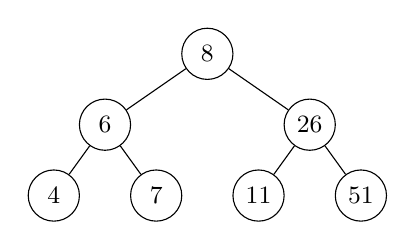
\begin{tikzpicture}[v/.style={circle,draw,minimum size=6.5mm,inner sep=0pt,font=\small},
  level distance=9mm, level 1/.style={sibling distance=26mm}, level 2/.style={sibling distance=13mm}]
\node[v] {8}
  child {node[v] {6} child {node[v] {4}} child {node[v] {7}}}
  child {node[v] {26} child {node[v] {11}} child {node[v] {51}}};
\end{tikzpicture}
\end{center}
用陣列存二元樹（資結書第~7.2.1~節）：根放第 $1$ 格，第 $i$ 格的左、右子節點放第 $2i$、$2i + 1$
格。 這棵樹是滿的，七格依層序是 $(8, 6, 26, 4, 7, 11, 51)$，選 c。

其他選項：
\begin{itemize}
\item a：照插入順序原封不動排，沒有建樹，也不是二元搜尋樹的樣子。 錯。
\item b：$26$ 的左子節點 $11$ 底下放了 $6$ 和 $4$ 兩個左右子節點，但 $4 < 6 < 11$，$4$ 不能是 $11$ 的右子
節點，連二元搜尋樹都不是。 錯。
\item d：這是插入 $4$ 時\textbf{沒有}做 LL 旋轉的樹 $26(8(6(4, 7), 11), 51)$ 的層序（而且省略了陣列裡空的
格子）。 這棵樹 $26$ 的左子樹高 $3$、右子樹高 $1$，不是 AVL 樹。 錯。
\item e：c 是對的。 錯。
\end{itemize}
\end{pastsoln}
